\documentclass[a4paper,12pt]{article}
\usepackage[UTF8]{ctex}
\usepackage{fullpage}  % leaves 1 inch margins all round
\usepackage{iftex}
\ifPDFTeX
  \usepackage[T1]{fontenc} % modern encoding (more characters available)
  \usepackage{mathptmx} % times in text and mathematics
  \usepackage[scaled]{helvet} % helvetica for sanserif, scaled 95% by default
  \usepackage{courier}  % for typewriter text
\else
  \usepackage{fontspec}
  \usepackage{unicode-math}
  \setmainfont{Times New Roman}
  \setsansfont{Arial}
  \setmonofont{Consolas}
  \setmathfont{Cambria Math}
\fi
\usepackage{textcomp} % lots of useful symbols
\usepackage{graphicx}  % inclusion of graphics files
\usepackage{amsmath}
\usepackage{cite}


\begin{document}

\title{How to write a technical project report}
\author{School of Engineering, University of Glasgow}
\date{\today}
 
\maketitle

\begin{abstract}
All reports start with an \emph{abstract}, which contains a summary of the project: its aim, what was done and what was achieved. This document describes the requirements for a project report in the department and gives advice on how to get better marks. It is structured to match a project report as far as possible.
\end{abstract}

%\tableofcontents

\section{Introduction}

\emph{Whew -- I've finished the work, now I only have to write the report.} Sound familar? Many students put off writing until too late and don't leave enough time to make a good job of the report. This is a serious mistake because the report typically accounts for a large fraction of the assessment. Start early -- most people find report-writing difficult. Think about the report throughout your project, keep track of references and collect material to illustrate the report.

\subsection{Mechanical aspects}

The length of the body of the report will be specified in the instructions for the project. Extra material may be provided in appendices but this material should be for reference only: you cannot assume that the reader will study it. In other words, do not put vital points in an appendix.

You will probably think that the report is too short but this is deliberate. Most reports are submitted to busy managers, who do not have time to read lengthy documents. It is important to learn how to pick out the vital points and write a concise report with maximum impact.

Reports should be word-processed and firmly bound. Use A4 paper and a clear typeface such as 12-point Times, number the pages and leave margins of at least 25\,mm all round. Follow this layout (this document breaks some of the rules to keep it compact).
\begin{itemize}
\item
The front cover should show the title of the project with your name(s) and matriculation number(s) and the name of your supervisor(s).
\item
Put the abstract on the next page. It should be about 100--250 words and gives a brief summary of the report including the background and aims of the project, the principal results and conclusions.
\item
The next page should show the table of contents. 
\item
The body of the report should be divided into numbered sections, each starting on a new page. Figures (diagrams, plots or photographs) and tables need captions and should be numbered.
\end{itemize}

\subsection{What goes into the introduction?}

Explain the background to the project and the reasons why your particular piece of work was considered worthwhile. This leads to the \textbf{aims} of the project: what you are trying to achieve. Be specific.


\section{Body of the report}

\subsection{实验协议与基本设置}

本文实验分为前后两个阶段。前期阶段主要用于搭建初始基线，并先看输入增强和损失函数设计会不会对分割表现带来实质变化。后期阶段则围绕 DRIVE 数据集 \cite{staal2004drive}，在统一的五折交叉验证设置下检验各项结构改进。由于两个阶段在数据来源、输入形式、划分方式和评价指标上都不相同，下面分开说明。

前期阶段对应前 3 次实验。这一阶段用多数据源样本训练最初版本的分割模型，同时测试较简单的输入增强和损失设计。后期主实验从第 4 次实验开始，第 4 次实验用于建立 DRIVE 上的统一基线；从第 5 次实验起，后续所有结构改进都沿用同一数据集、预处理流程和五折划分，因此横向比较更直接。

\subsubsection{数据集与数据组织}

在前期探索阶段，训练数据来自多个公开视网膜血管分割数据集，包括 STARE \cite{hoover2000locating}、CHASE\_DB1 \cite{fraz2012ensemble} 和 HRF \cite{budai2013robust}。前 3 次实验没有重新划分数据，而是直接沿用师兄留下的训练集和验证集列表。这样做的好处是可以和前期工作在同一条件下直接比较。按照现有划分文件，训练集和验证集样本数分别为 801 和 90。

前期输入采用三通道分离方式。原始彩色眼底图像先转换为 nnU-Net 可读取的 NIfTI 格式，再拆成红、绿、蓝三个独立通道分别输入模型。这样既保留了原始图像的光谱信息，也方便后面分析不同颜色通道，尤其是绿色通道，以及对比度增强策略的作用。

后期实验只使用 DRIVE，并统一使用同一套数据组织流程。输入不再是三通道彩色图像，而是将原始眼底图像依次做灰度化、标准化、自适应直方图均衡化和 gamma 校正，再保存为单通道 NIfTI 文件。这个预处理流程参考了 PA-Net \cite{luo2025panet} 的设置。实际效果上，它更有利于突出细小血管和低对比区域，同时减少颜色信息带来的无关干扰。

从第 4 次实验开始，后期实验的数据组织和五折划分都保持不变。因此，后面各模型之间的性能差异主要可以归因于网络结构、损失函数或后处理策略，而不是数据划分本身。

\subsubsection{实现细节与评价指标}

全部实验基于 nnU-Net v2 框架实现 \cite{isensee2021nnunet}。同一阶段内，除非某项改动本身就是实验变量，否则训练流程保持一致。后期实验主要调整的是 nnU-Net 中 U-Net 主体结构以及不同阶段之间的特征交互方式，只有少数实验会改动损失函数或 trainer 层面的训练策略。前期阶段用固定划分验证方案可行性，后期阶段则在 DRIVE 上采用 2D nnU-Net 配置和五折交叉验证来评估结构改动。

前期阶段的基线模型使用标准 nnU-Net 训练器，训练 150 个 epoch。前 3 次实验分别对应原始输入的 baseline、加入 CLAHE 的输入增强版本，以及在 CLAHE 基础上叠加 Dice loss 与 Focal Loss 的版本。该阶段评价脚本输出 IoU (vessel)、mIoU、Recall、Precision、Accuracy、mPA 和 F1-score，前期结果均按这组指标报告。

后期主实验统一使用 nnU-Net v2 的 2D 配置，输入 patch size 为 \(512 \times 512\)，batch size 为 2，训练 100 个 epoch。优化器采用 SGD，初始学习率 0.001，并使用 Poly 学习率衰减。除特别说明外，所有模型都沿用同一数据划分和训练计划。第 4 次实验是这一阶段的基线，第 5 次实验及其后的结构变体都在这套设置下比较。

评估时，后期阶段不依赖单个 fold 的结果，而是把五折验证输出合并后再统一计算指标。每个 fold 负责其验证子集的预测，最终指标在完整交叉验证输出上统计。这样可以减少单次划分带来的偶然波动，也让模型间比较更稳。

后期阶段报告的指标包括 Sensitivity (SE)、Specificity (SP)、Accuracy (ACC)、AUC、Precision (PR) 和 F1-score。SE 主要反映细小血管和弱响应区域的检出情况，SP 和 PR 用来观察伪阳性的控制程度，ACC 表示整体像素分类准确率，F1-score 用于概括整体分割质量。由于当前实验没有保存概率图，AUC 由二值预测结果近似计算。

\subsection{基线与前期探索}

前 3 次实验更像是正式结构改动前的一轮摸底。它们直接沿用既有训练集和验证集名单，以便和刘师兄的实验设置保持一致，也方便在同样数据条件下做对照。三次实验都以 DRIVE 为测试集，并使用同一组前期评价指标。

第一次实验采用标准 nnU-Net 基线模型 \cite{isensee2021nnunet}。在固定划分下，它已经能给出比较稳定的整体分割结果，因此可以作为后续实验的参照。

第二次实验在同样训练框架下加入 CLAHE。结果显示，训练前期收敛更快了，但最终分割指标提升并不明显。换句话说，单靠把输入变“更清楚”，还不足以真正解决细小血管和复杂分叉区域的建模问题。

第三次实验在 CLAHE 基础上再引入 Focal Loss，希望让模型更关注困难像素和类别不平衡问题。它确实让收敛进一步加快，但最终性能提升仍不稳定。这也说明，在当前网络结构下，单改损失函数还不足以可靠地把结果推过基线。

把这三次实验放在一起看，结论其实比较明确：输入增强和损失函数设计会影响训练过程，也会带来局部指标变化，但它们并没有真正改变模型处理细小血管、低对比区域和结构连续性的方式。所以后面的工作不再停留在训练层面的小修小补，而是转向结构改进。

\begin{table}[htbp]
\centering
\caption{前期探索实验结果汇总}
\label{tab:early_experiments}
\begin{tabular}{llllll}
\hline
实验编号 & 方法 & 训练设置 & 收敛情况 & 代表性结果 & 主要观察 \\
\hline
Exp1 & nnU-Net baseline & Dice, 150 epoch & 第69个 epoch 收敛 & F1 = 0.7924 & 建立前期基线 \\
Exp2 & CLAHE + nnU-Net & Dice, 150 epoch & 第60个 epoch 收敛 & F1 = 0.7827 & 改善早期收敛，但最终提升有限 \\
Exp3 & CLAHE + nnU-Net + Focal Loss & Focal Loss, 150 epoch & 第53个 epoch 收敛 & F1 = 0.7802 & 收敛更快，但性能未进一步提升 \\
\hline
\end{tabular}
\end{table}

\subsection{PA-Net 模块迁移}

完成基线和前期探索后，下一步是把 PA-Net 的两个核心模块迁到 nnU-Net 中，即 Lightweight Parallel Transformer (LPT) 和 Adaptive Vascular Feature Fusion Module (AFFM) \cite{luo2025panet}。这里的目的不是立刻得到最终模型，而是先看 PA-Net 的关键设计在当前任务里是否好用，以及哪些部分值得继续保留。

LPT 放在网络 bottleneck 位置，用来补强长程依赖和全局血管结构的建模。PA-Net 中的 LPT 把局部特征处理和并行注意力结合在一起，计算开销不算高，但能扩大特征交互范围。对视网膜血管分割来说，这有助于模型在高层特征里保留更完整的血管走向，尤其是在细小血管容易断裂或消失的地方。AFFM 则替代标准的 skip connection 融合方式，不再直接拼接，而是通过自适应加权让不同层级的特征参与解码。这样浅层细节和深层语义可以分工更明确。对于当前任务，我们希望它能减少下采样带来的细节损失，并改善边缘和分叉区域的恢复。

从抽象计算形式上看，若将输入特征记为 \(X\)，则 LPT 中的注意力分支可以写为
\[
Q = XW_Q,\qquad K = XW_K,\qquad V = XW_V,
\]
\[
\mathcal{A}(X) = \mathrm{Softmax}\left(\frac{QK^{\top}}{\sqrt{d}}\right)V,
\]
其中 \(d\) 表示特征维度。若进一步将局部分支记为 \(\mathcal{L}(X)\)，则 LPT 的输出可以概括为
\[
Y_{\mathrm{LPT}} = \mathrm{FFN}\big(\mathcal{L}(X) + \mathcal{A}(X)\big) + X.
\]
这一形式说明，LPT 的核心并不只是引入注意力，而是将局部特征提取与全局依赖建模并行结合后再进行融合。对于 AFFM，若将来自三个层级的输入特征分别记为 \(F_1\)、\(F_2\) 和 \(F_3\)，则其融合过程可以简化表示为
\[
Y_{\mathrm{AFFM}} = \sum_{i=1}^{3}\alpha_i \odot F_i,\qquad
[\alpha_1,\alpha_2,\alpha_3] = \mathrm{Softmax}\big(\phi([F_1,F_2,F_3])\big),
\]
其中 \(\phi(\cdot)\) 表示由卷积映射得到的权重生成函数，\(\odot\) 表示逐元素加权。这一表达式更直接地说明了 AFFM 的作用：解码阶段不会把不同层的特征一视同仁，而是根据当前内容重新分配它们的权重。

\begin{figure}[htbp]
\centering
\begin{minipage}{0.4\textwidth}
\centering
\includegraphics[height=0.22\textheight,keepaspectratio]{pic/panet.png}\\
(a) PA-Net 整体结构
\end{minipage}
\hfill
\begin{minipage}{0.2\textwidth}
\centering
\includegraphics[height=0.22\textheight,keepaspectratio]{pic/LPT.png}\\
(b) LPT 模块结构
\end{minipage}
\hfill
\begin{minipage}{0.33\textwidth}
\centering
\includegraphics[height=0.22\textheight,keepaspectratio]{pic/AFFM.png}\\
(c) AFFM 模块结构
\end{minipage}
\caption{PA-Net 及其迁移到 nnU-Net 的两个核心模块。三幅图采用相同高度以便于横向比较。}
\label{fig:panet_triplet}
\end{figure}

这一阶段先把 LPT 和 AFFM 一起引入 nnU-Net，并在统一协议下与基线比较，先看完整迁移后的整体效果。由于后续实验主要围绕 U-Net 主体结构和特征交互方式展开，这个版本也自然成为后面做消融和继续改结构的起点。下一节便分别考察 LPT 与 AFFM 的单独作用。

\subsection{LPT 与 AFFM 的消融}

把 PA-Net 风格的完整迁移搭起来之后，接下来最需要回答的问题就是：性能变化到底主要来自哪个模块。为此，本节继续沿用后期主实验的统一设置，包括相同的单通道预处理、相同的五折划分和相同的 DRIVE 训练计划。和前文一样，指标基于五折验证结果汇总后计算，而不是看某一个 fold。

考虑到 nnU-Net 与主干结构耦合较紧，本节在基线之外又构建了三组模型：完整 PA-Net 迁移、只引入 LPT 的 LPT Only，以及只引入 AFFM 的 AFFM Only。其中 LPT Only 对应消融 A，只在 bottleneck 处加入 LPT；AFFM Only 对应消融 B，只替换解码阶段的特征融合。

\begin{table}[htbp]
\centering
\caption{LPT 与 AFFM 消融实验结果对比}
\label{tab:lpt_affm_ablation}
\resizebox{\textwidth}{!}{
\begin{tabular}{lcccccc}
\hline
实验组 & SE & SP & ACC & AUC & PR & F1-score \\
\hline
nnU-Net v2 Baseline & $0.7627 \pm 0.0446$ & $0.9852 \pm 0.0050$ & $0.9659 \pm 0.0045$ & $0.8739 \pm 0.0210$ & $0.8238 \pm 0.0646$ & $0.7891 \pm 0.0320$ \\
PA-Net (Full) & $0.7211 \pm 0.0763$ & $0.9888 \pm 0.0050$ & $0.9659 \pm 0.0059$ & $0.8549 \pm 0.0365$ & $0.8570 \pm 0.0621$ & $0.7782 \pm 0.0464$ \\
LPT Only (消融 A) & $0.7597 \pm 0.0492$ & $0.9864 \pm 0.0041$ & $0.9669 \pm 0.0044$ & $0.8731 \pm 0.0234$ & $0.8361 \pm 0.0546$ & $0.7935 \pm 0.0297$ \\
AFFM Only (消融 B) & $0.7573 \pm 0.0475$ & $0.9868 \pm 0.0039$ & $0.9672 \pm 0.0045$ & $0.8720 \pm 0.0227$ & $0.8400 \pm 0.0517$ & $0.7942 \pm 0.0300$ \\
\hline
\end{tabular}
}
\end{table}

表 \ref{tab:lpt_affm_ablation} 给出的趋势其实比较清楚。完整 PA-Net 迁移并没有超过基线，反倒是两个单模块版本整体更稳。LPT Only 在基本不损失 SE 的情况下，小幅提高了 PR 和 F1-score，说明 LPT 至少值得继续往下做。AFFM Only 虽然在这组对比里拿到了最高的 ACC 和 F1-score，但领先幅度有限，还不足以让它成为后续实验的主方向。

因此，这一节更像是在缩小问题范围。PA-Net 里的某些单独设计仍有参考价值，但把 LPT 和 AFFM 一起迁进 nnU-Net，并没有得到更好的整体结构。本节的主要作用不是立刻确定最终路线，而是先判断性能下滑可能出在哪些环节。接下来的实验便转向更细地看模块本身，以及它们和现有训练机制之间的关系。更细的指标分析放在第三章讨论。

\subsection{AFFM 与深监督的兼容性验证}

AFFM 在 PA-Net 中负责解码阶段的多层特征融合 \cite{luo2025panet}，而 nnU-Net 的深监督也作用在解码器的多尺度特征上 \cite{isensee2021nnunet,lee2015dsn}。两者都落在相近的位置，所以这里额外做了一组控制实验，想看它们在当前框架下会不会互相冲突。实验仍沿用后期统一设置，即相同的单通道预处理、五折划分和 DRIVE 训练计划，指标也还是在五折结果汇总后计算。

在 nnU-Net 的默认训练流程中，深监督会在解码器的多个阶段施加辅助分割损失，以强化多尺度特征学习 \cite{isensee2021nnunet,lee2015dsn}。若将主输出损失记为 \(\mathcal{L}_{\mathrm{main}}\)，将第 \(s\) 个辅助输出损失记为 \(\mathcal{L}_{\mathrm{aux}}^{(s)}\)，则总损失可以写为
\[
\mathcal{L} = \mathcal{L}_{\mathrm{main}} + \sum_{s=1}^{S}\lambda_s \mathcal{L}_{\mathrm{aux}}^{(s)},
\]
其中 \(\lambda_s\) 表示各辅助分支的权重。图 \ref{fig:deep_supervision_cn} 展示了深监督的基本方式：训练时在多个解码层挂辅助分割头共同参与损失计算，推理时只保留主输出。为了判断前一节看到的性能变化是否与深监督有关，本节在 AFFM Only 的基础上关闭深监督，构造了 AFFM w/o DS，并与保留深监督的版本做对比。

\begin{figure}[htbp]
\centering
\includegraphics[width=0.95\textwidth]{pic/deep_supervision.png}
\caption{nnU-Net 解码器中深监督机制的示意图。训练阶段在多个解码层附加辅助分割头并共同计算加权总损失，而推理阶段仅保留主输出。}
\label{fig:deep_supervision_cn}
\end{figure}

\begin{table}[htbp]
\centering
\caption{AFFM 在有无深监督下的结果对比}
\label{tab:affm_ds_cn}
\resizebox{\textwidth}{!}{
\begin{tabular}{lcccccc}
\hline
实验组 & SE & SP & ACC & AUC & PR & F1-score \\
\hline
AFFM Only (with DS) & $0.7573 \pm 0.0475$ & $0.9868 \pm 0.0039$ & $0.9672 \pm 0.0045$ & $0.8720 \pm 0.0227$ & $0.8400 \pm 0.0517$ & $0.7942 \pm 0.0300$ \\
AFFM w/o DS & $0.7401 \pm 0.0493$ & $0.9880 \pm 0.0038$ & $0.9667 \pm 0.0048$ & $0.8640 \pm 0.0236$ & $0.8490 \pm 0.0534$ & $0.7883 \pm 0.0308$ \\
\hline
\end{tabular}
}
\end{table}

结果比较直接。关闭深监督后，SP 和 PR 略有上升，但 SE、AUC 和 F1-score 都下降了。也就是说，模型变得更保守了，伪阳性少了一些，但细小血管和弱响应区域也更容易漏掉。

所以，去掉深监督并没有把 AFFM 这条路线“救回来”。它最多解释了精度变化的一部分，解释不了前面看到的整体趋势。这组实验的价值主要在于先排除一个可能原因，并进一步说明 AFFM 在当前框架下的收益并不稳定。至于 AFFM 之后还要不要保留，仍要看后续结构实验的结果。更细的讨论放在第三章。

\subsection{LPT 中的可变形注意力}

在做完 AFFM 与深监督关系的控制实验之后，关注点重新回到了 LPT 本身。本节想回答的是：能不能通过改写 LPT 的高层特征建模方式，把这条路线继续往前推。具体做法是参考可变形注意力 \cite{zhu2021deformabledetr}，用它替换 PA-Net 中 LPT 原有的 GAA 形式 \cite{luo2025panet}。这样做的考虑很现实：视网膜血管往往是弯曲的，还有分叉和细小末梢，用刚性的固定采样并不容易贴合这类结构。实验依然使用后期统一的 DRIVE 设置，指标来自五折输出的汇总结果。

与 GAA 中较为规则的固定采样方式不同，可变形注意力通过为参考位置学习若干偏移量，使特征聚合能够更灵活地分布在目标结构周围。若将参考位置记为 \(p\)，第 \(k\) 个采样偏移记为 \(\Delta p_k\)，对应权重记为 \(A_k\)，则其局部聚合过程可以写为
\[
\mathrm{DefAttn}(p) = \sum_{k=1}^{K} A_k \cdot x(p + \Delta p_k),\qquad
\sum_{k=1}^{K} A_k = 1,
\]
其中 \(K\) 表示采样点数。对血管分割来说，这意味着采样位置不必再拘泥于固定方向，而是可以更自然地贴合弯曲血管、分叉和细小末梢的真实走向。图 \ref{fig:deformable_attention_cn} 展示了 GAA 与可变形注意力的采样差异，其中 4 point 和 8 point 仅表示每个参考位置周围参与聚合的采样点数。

\begin{figure}[htbp]
\centering
\includegraphics[width=0.95\textwidth]{pic/Deformable_Attention.png}
\caption{GAA 与可变形注意力采样方式的示意对比。左图表示较为规则的固定采样，右图表示围绕参考位置进行自适应偏移的采样方式。}
\label{fig:deformable_attention_cn}
\end{figure}

本节首先构建不含 AFFM 的 Deformable LPT（4 point），单独看可变形注意力替换本身是否有效；随后在相同设置下把 AFFM 加回去，检查 LPT 改写后它是否还有保留价值；最后再把采样点数从 4 point 扩到 8 point，观察更大采样规模是否带来收益。表 \ref{tab:deformable_lpt_cn} 汇总了这组实验结果。

\begin{table}[htbp]
\centering
\caption{可变形 LPT 相关实验结果对比}
\label{tab:deformable_lpt_cn}
\resizebox{\textwidth}{!}{
\begin{tabular}{lcccccc}
\hline
实验组 & SE & SP & ACC & AUC & PR & F1-score \\
\hline
LPT Only & $0.7597 \pm 0.0492$ & $0.9864 \pm 0.0041$ & $0.9669 \pm 0.0044$ & $0.8731 \pm 0.0234$ & $0.8361 \pm 0.0546$ & $0.7935 \pm 0.0297$ \\
Deformable LPT (No AFFM, 4 point) & $0.7634 \pm 0.0540$ & $0.9863 \pm 0.0043$ & $0.9672 \pm 0.0044$ & $0.8749 \pm 0.0254$ & $0.8371 \pm 0.0511$ & $0.7958 \pm 0.0275$ \\
Deformable LPT + AFFM & $0.7571 \pm 0.0495$ & $0.9867 \pm 0.0042$ & $0.9670 \pm 0.0044$ & $0.8719 \pm 0.0235$ & $0.8388 \pm 0.0545$ & $0.7933 \pm 0.0301$ \\
Deformable LPT (No AFFM, 8 point) & $0.7573 \pm 0.0506$ & $0.9869 \pm 0.0038$ & $0.9672 \pm 0.0047$ & $0.8721 \pm 0.0241$ & $0.8412 \pm 0.0504$ & $0.7946 \pm 0.0296$ \\
\hline
\end{tabular}
}
\end{table}

这组结果里，最清楚的提升来自不含 AFFM 的 Deformable LPT（4 point）。和 LPT Only 相比，它在 SE、AUC 和 F1-score 上都有提升，说明 bottleneck 处更灵活的采样方式确实有助于高层血管结构建模。相比继续围绕 AFFM 调整，这条路线更值得往下做。

把 AFFM 重新加回来之后，结果并没有继续变好。Deformable LPT + AFFM 的 F1-score 反而从 0.7958 降到 0.7933，可见在新的 LPT 结构下，AFFM 依旧没有表现出稳定增益。从这一阶段开始，后续实验便不再保留 AFFM，而是沿着改进后的 LPT 路线继续推进。

4 point 和 8 point 的比较也很有意思。8 point 虽然让 PR 略有上升，但在 SE、AUC 和 F1-score 上都没有超过 4 point。换句话说，采样点变多并没有自动带来更好的整体结果。因此，后续实验优先保留不含 AFFM 的 Deformable LPT（4 point）作为基础设置。更细的分析将在第三章展开。

\subsection{Modulated 与多尺度可变形 LPT}

在确定不含 AFFM 的 Deformable LPT（4 point）可以作为后续基础后，下面的实验沿两个方向继续推进。第一条是参考调制可变形机制 \cite{zhu2019dcnv2}，在单尺度可变形采样里加入 modulation mask，希望压低无关响应、让模型更聚焦于真正重要的采样点。第二条是参考多尺度可变形注意力 \cite{zhu2021deformabledetr}，把 bottleneck 的采样范围从当前层扩展到 encoder 的多层特征上，看看跨层聚合能不能补回一部分高分辨率细节。实验仍使用后期统一的 DRIVE 设置，指标来自五折结果汇总。

若以前一节中的单尺度可变形采样为基础，将第 \(k\) 个采样点的 modulation mask 记为 \(m_k\)，则单尺度 modulated deformable 形式可以写为
\[
\mathrm{ModDefAttn}(p) = \sum_{k=1}^{K} m_k A_k \cdot x(p + \Delta p_k),\qquad
m_k = \sigma(g_k(x)),
\]
其中 \(\sigma(\cdot)\) 表示 Sigmoid 函数，\(g_k(\cdot)\) 表示掩码生成映射。图 \ref{fig:modulated_deformable_cn} 给出了单尺度 Modulated Deformable 采样的示意图，其中 modulation mask 用于进一步调节不同采样点在聚合中的贡献。进一步地，若将多尺度输入特征记为 \(\{x_l\}_{l=1}^{L}\)，并记第 \(l\) 层的线性映射为 \(P_l(\cdot)\)，则多尺度 modulated deformable 聚合可概括为
\[
\mathrm{MSModDefAttn}(p) = \sum_{l=1}^{L}\sum_{k=1}^{K} A_{l,k} m_{l,k} \cdot P_l\big(x_l(p_l + \Delta p_{l,k})\big).
\]
这个表达式对应的变化不只是“采样点更多了”。真正变化的是 bottleneck 特征可以把当前层作为 query，同时跨层访问 encoder 的多级特征并进行加权聚合。图 \ref{fig:ms_modulated_cn} 展示了这一跨层多尺度采样与聚合的整体过程。

\begin{figure}[htbp]
\centering
\includegraphics[width=0.9\textwidth]{pic/Modulated_Deformable_Sampling.png}
\caption{单尺度 Modulated Deformable 采样示意图。查询点通过可变形偏移访问周围采样位置，并利用 modulation mask 对不同采样点的贡献进行进一步调节。}
\label{fig:modulated_deformable_cn}
\end{figure}

\begin{figure}[htbp]
\centering
\includegraphics[width=0.95\textwidth]{pic/MS_modulated_DF.png}
\caption{多尺度 Modulated Deformable 采样示意图。bottleneck 特征作为 query，跨层访问 encoder 多尺度特征，并通过加权聚合形成增强后的 bottleneck 表示。}
\label{fig:ms_modulated_cn}
\end{figure}

基于这个思路，本节先构建不含 AFFM 的 Modulated Deformable（4 point），单独看 modulation mask 的作用；再构建 MS-Modulated（4 point），检验跨层多尺度采样能否在保留可变形采样灵活性的同时补进更多浅层细节。表 \ref{tab:modulated_msdeform_cn} 给出了结果。

\begin{table}[htbp]
\centering
\caption{Modulated 与多尺度可变形 LPT 实验结果对比}
\label{tab:modulated_msdeform_cn}
\resizebox{\textwidth}{!}{
\begin{tabular}{lcccccc}
\hline
实验组 & SE & SP & ACC & AUC & PR & F1-score \\
\hline
Deformable LPT (No AFFM, 4 point) & $0.7634 \pm 0.0540$ & $0.9863 \pm 0.0043$ & $0.9672 \pm 0.0044$ & $0.8749 \pm 0.0254$ & $0.8371 \pm 0.0511$ & $0.7958 \pm 0.0275$ \\
Deformable LPT (No AFFM, 8 point) & $0.7573 \pm 0.0506$ & $0.9869 \pm 0.0038$ & $0.9672 \pm 0.0047$ & $0.8721 \pm 0.0241$ & $0.8412 \pm 0.0504$ & $0.7946 \pm 0.0296$ \\
Modulated Deformable (4 point) & $0.7660 \pm 0.0511$ & $0.9858 \pm 0.0048$ & $0.9669 \pm 0.0046$ & $0.8759 \pm 0.0241$ & $0.8324 \pm 0.0560$ & $0.7950 \pm 0.0305$ \\
MS-Modulated (4 point) & $0.7582 \pm 0.0509$ & $0.9870 \pm 0.0038$ & $0.9673 \pm 0.0046$ & $0.8726 \pm 0.0242$ & $0.8419 \pm 0.0497$ & $0.7954 \pm 0.0283$ \\
\hline
\end{tabular}
}
\end{table}

这两个变体改善的方向并不一样。Modulated Deformable（4 point）在本组里拿到了最高的 SE 和 AUC，更像是在说明 modulation mask 提升了模型对细小血管和弱响应区域的检出能力。额外的选择机制确实改变了采样分布，让模型更愿意关注与血管连续性相关的位置。

MS-Modulated（4 point）则呈现出另一种特点。它没有继续提高 SE，但在 SP、ACC 和 PR 上更好，这说明跨层多尺度采样更擅长抑制背景噪声，并让整体预测更平衡。换句话说，这一步的收益更多来自不同层级信息的补充和整合，而不是单纯把灵敏度往上推。

因此，本节的结论不是哪一个版本彻底胜出，而是两者各自把模型往不同方向推了一步。modulation mask 更偏向提升血管检出，多尺度扩展更偏向改善整体平衡。虽然它们都没有在 F1-score 上明显超过上一节的 Deformable LPT（4 point），但至少把后续设计取舍看得更清楚了。更细的指标讨论将在第三章展开。

\subsection{MS-Modulated 与 Coordinate Attention}

做完 modulation 和多尺度可变形采样之后，下一步是在 MS-Modulated 上加入 Coordinate Attention (CA) \cite{hou2021coordatt}。原因很直接：视网膜血管细、长，而且方向性很强，CA 恰好能够在保留长程依赖的同时显式保留位置信息。它和普通通道注意力不同，会沿水平方向和垂直方向分别聚合特征，因此对空间位置更敏感。本节仍使用后期统一设置，指标来自五折结果汇总。

若将输入特征记为 \(X \in \mathbb{R}^{C\times H\times W}\)，则 CA 可以先沿两个空间方向分别进行聚合，得到
\[
z_h(c,h)=\frac{1}{W}\sum_{i=1}^{W}X(c,h,i),\qquad
z_w(c,w)=\frac{1}{H}\sum_{j=1}^{H}X(c,j,w).
\]
经过共享映射和方向相关变换后，可得到两个方向敏感的注意力图 \(a_h\) 和 \(a_w\)，其输出可以概括为
\[
Y_{\mathrm{CA}} = X \odot a_h \odot a_w.
\]
这个表达式说明，CA 不是拿来替代多尺度可变形采样的，而是在其基础上按方向和位置重新分配特征响应。图 \ref{fig:ms_ca_cn} 给出了两者结合后的整体结构。

\begin{figure}[htbp]
\centering
\includegraphics[width=0.95\textwidth]{pic/MS_CA.png}
\caption{MS-Modulated 与 Coordinate Attention 结合的结构示意图。多尺度可变形采样先完成跨层信息聚合，随后由 Coordinate Attention 在空间方向上进一步重标定特征响应。}
\label{fig:ms_ca_cn}
\end{figure}

本节以 MS-Modulated（4 point）为直接对照，在其上加入 CA，构造 MS-Modulated + CA，想看显式位置注意力能否让跨层可变形采样的表现更稳。表 \ref{tab:msmod_ca_cn} 给出了结果。

\begin{table}[htbp]
\centering
\caption{MS-Modulated 与 MS-Modulated + CA 实验结果对比}
\label{tab:msmod_ca_cn}
\resizebox{\textwidth}{!}{
\begin{tabular}{lcccccc}
\hline
实验组 & SE & SP & ACC & AUC & PR & F1-score \\
\hline
nnU-Net v2 (Baseline) & $0.7627$ & $0.9852$ & $0.9659$ & $0.8739$ & $0.8238$ & $0.7891$ \\
Modulated (单尺度, 4 point) & $0.7660$ & $0.9858$ & $0.9669$ & $0.8759$ & $0.8324$ & $0.7950$ \\
MS-Modulated (4 point) & $0.7582$ & $0.9870$ & $0.9673$ & $0.8726$ & $0.8419$ & $0.7954$ \\
MS-Modulated + CA & $0.7697$ & $0.9857$ & $0.9673$ & $0.8777$ & $0.8324$ & $0.7973$ \\
\hline
\end{tabular}
}
\end{table}

加入 CA 后，SE、AUC 和 F1-score 都有所提升，分别达到 0.7697、0.8777 和 0.7973。这个结果说明，CA 确实帮助模型更好地找回了细小血管和弱响应区域，同时没有破坏整体分割质量。

和上一节对照来看，MS-Modulated 本身更擅长提高 SP、ACC 和 PR，而 CA 的加入则把 SE、AUC 和 F1-score 往上推了一步。因此，CA 的作用不只是继续压伪阳性，更重要的是在保持整体稳定的同时，帮助模型恢复细长血管结构。可以把它理解为：多尺度可变形采样负责做跨层信息交互，CA 负责让这些信息在空间上表达得更有选择性。

到这一阶段，MS-Modulated + CA 已经是当前序列里综合表现最好的结果，也自然成为下一步继续改结构的过渡版本。这一步也说明，即便可变形采样已经足够灵活，显式保留方向和位置信息仍然是有价值的。更细的比较放在第三章讨论。

\subsection{MS-DSConv 与 CA}

得到 MS-Modulated + CA 后，一个新问题也变得更明显了。多尺度可变形采样和 CA 确实增强了跨层信息交互与位置选择，但当前采样方式本质上还是离散点式的。它能找到关键位置，却未必擅长描述视网膜血管这种细长、连续、弯曲的几何形态。基于这一点，后续实验引入动态蛇形卷积（Dynamic Snake Convolution, DSConv）\cite{qi2023dsc}，希望让相邻采样点之间形成连续轨迹，从而让采样路径更贴近真实血管走向。需要说明的是，这一步并不是把全网普通卷积都替换掉，而是只把 DSConv 用在 bottleneck 处 LPT 的多尺度采样分支上，用来替代上一阶段 MS-Modulated 中的离散式跨层可变形采样。实验设置仍与后期 DRIVE 协议保持一致，指标基于五折结果汇总。

与前面可变形注意力中各采样点相对独立的形式不同，动态蛇形卷积的关键在于让后续采样位置依赖前面位置的偏移结果。若将第 \(k\) 个采样点的纵向增量记为 \(\delta y_k\)，横向基础步长记为 \(\Delta x_k\)，则蛇形轨迹上的采样位置可以概括为
\[
\tilde{p}_k = p + \left(\Delta x_k,\; \sum_{t=1}^{k}\delta y_t\right).
\]
在多尺度场景下，若进一步将第 \(l\) 个尺度上的聚合写为
\[
\mathrm{MSDSConv}(p) = \sum_{l=1}^{L}\sum_{k=1}^{K} A_{l,k} m_{l,k}\cdot P_l\big(x_l(\tilde{p}_{l,k})\big),
\]
和前面的多尺度 modulated deformable 相比，最大的区别在于采样点不再被视为彼此独立的离散位置，而是沿着一条连续展开的轨迹聚合。这种形式更适合刻画血管的弯曲、连通和拓扑连续性。图 \ref{fig:msds_ca_cn} 展示了 MS-DSConv 与 CA 结合后的整体结构。

\begin{figure}[htbp]
\centering
\includegraphics[width=0.95\textwidth]{pic/MSDS.png}
\caption{MS-DSConv 与 Coordinate Attention 结合的结构示意图。多尺度采样分支中的采样点沿连续蛇形轨迹展开，在完成跨层加权聚合后，再由 Coordinate Attention 对空间响应进行进一步重标定。}
\label{fig:msds_ca_cn}
\end{figure}

本节以 MS-Modulated + CA 为直接对照，构建 MS-DSConv + CA，想检验连续轨迹建模能否进一步提高细小血管恢复能力和整体结构完整性。表 \ref{tab:msdsconv_ca_cn} 汇总了结果。

\begin{table}[htbp]
\centering
\caption{MS-Modulated + CA 与 MS-DSConv + CA 实验结果对比}
\label{tab:msdsconv_ca_cn}
\resizebox{\textwidth}{!}{
\begin{tabular}{lcccccc}
\hline
实验组 & SE & SP & ACC & AUC & PR & F1-score \\
\hline
nnU-Net v2 (Baseline) & $0.7627$ & $0.9852$ & $0.9659$ & $0.8739$ & $0.8238$ & $0.7891$ \\
MS-Modulated (4 point) & $0.7582$ & $0.9870$ & $0.9673$ & $0.8726$ & $0.8419$ & $0.7954$ \\
MS-Modulated + CA & $0.7697$ & $0.9857$ & $0.9673$ & $0.8777$ & $0.8324$ & $0.7973$ \\
MS-DSConv + CA & $0.8083$ & $0.9815$ & $0.9666$ & $0.8949$ & $0.7997$ & $0.8020$ \\
\hline
\end{tabular}
}
\end{table}

这一改动带来的提升比较明显。加入 DSConv 后，SE、AUC 和 F1-score 分别提高到 0.8083、0.8949 和 0.8020。也就是说，从独立点式采样转向轨迹式采样之后，模型在连接细小血管、修复断裂区域以及保留连续拓扑方面确实更强了。

当然，代价也存在。MS-DSConv + CA 的 SP 和 PR 比上一节略低，说明这种更强调几何连续性的建模方式也会把更多潜在血管像素一起检出来，因此引入了一些额外伪阳性。即便如此，从整体指标看，这个代价仍然是值得的，因为视网膜血管分割更在意连续细血管能不能被保留下来，而不只是把结果做得尽可能“干净”。

在这一阶段，MS-DSConv + CA 给出了目前最好的结果。更重要的是，它把关注点从“采样点选在哪”和“跨层怎么融合”进一步推进到了“血管连续性本身怎么建模”。这也使它自然成为最后一步精修的基础版本。不过，它偏低的 PR 也提示我们，预测结果里仍然有一些误检区域，所以接下来需要引入小连通域后处理。

\subsection{小连通域后处理}

即便 MS-DSConv + CA 已经是当前最好的模型，仍有一个问题没有解决：PR 还低于 0.8。这通常意味着二值预测图里还留着一些小噪声连通域和伪阳性区域。为此，后续实验加入了一个简单的小连通域后处理规则。网络主体不再改动，只在输出分割图上按面积阈值移除孤立小区域，同时尽量保留主要血管结构。

若将预测结果中的一个连通域记为 \(C_i\)，其像素面积记为 \(|C_i|\)，面积阈值记为 \(X\)，则后处理规则可以简化表示为
\[
\hat{Y}_{\mathrm{post}}(C_i)=
\begin{cases}
1, & |C_i| \ge X,\\
0, & |C_i| < X.
\end{cases}
\]
其中，\(X=0\) 表示不做后处理；\(X\) 越大，被移除的小连通域就越多。图 \ref{fig:postprocess_threshold_cn} 展示了不同阈值下主要指标的变化趋势，表 \ref{tab:postprocess_cn} 给出了对应实验结果。

\begin{figure}[htbp]
\centering
\includegraphics[width=0.9\textwidth]{pic/Postprocess_Threshold_Metrics_dual_axis.png}
\caption{后处理面积阈值对主要指标的影响。左侧纵轴表示 SE、PR 和 F1-score，右侧纵轴表示 SP，用于更清楚地展示不同量级指标随阈值变化的趋势。}
\label{fig:postprocess_threshold_cn}
\end{figure}

\begin{table}[htbp]
\centering
\caption{MS-DSConv + CA 在不同后处理阈值下的结果对比}
\label{tab:postprocess_cn}
\resizebox{\textwidth}{!}{
\begin{tabular}{lcccccc}
\hline
实验组 & SE & SP & ACC & AUC & PR & F1-score \\
\hline
MS-DSConv + CA ($X=0$) & $0.8083$ & $0.9815$ & $0.9666$ & $0.8949$ & $0.7997$ & $0.8020$ \\
MS-DSConv + CA ($X=20$) & $0.8059$ & $0.9819$ & $0.9668$ & $0.8939$ & $0.8035$ & $0.8027$ \\
MS-DSConv + CA ($X=30$) & $0.8046$ & $0.9821$ & $0.9669$ & $0.8933$ & $0.8048$ & $0.8026$ \\
MS-DSConv + CA ($X=90$) & $0.7995$ & $0.9827$ & $0.9670$ & $0.8911$ & $0.8089$ & $0.8021$ \\
\hline
\end{tabular}
}
\end{table}

这组阈值实验反映的是一个很典型的权衡。\(X=0\) 时不做后处理，模型保留了最强的血管检出能力，SE、AUC 和 F1-score 分别为 0.8083、0.8949 和 0.8020，但 PR 只有 0.7997，说明误检区域确实还在。随着阈值提高到 20、30 和 90，SP、PR 和 ACC 逐步上升，而 SE 和 AUC 逐步下降。也就是说，后处理确实清掉了一部分噪声，但同时也开始删掉真实的细小血管。

\(X=20\) 时 F1-score 最高，为 0.8027，看起来是在去除伪阳性和保留细血管之间比较平衡的一档。\(X=30\) 时 PR 和 SP 更高，结果也更干净、更保守。到了 \(X=90\)，PR 虽然升到 0.8089，但 SE 已降到 0.7995，说明阈值过大时已经开始误删真实血管，尤其是面积较小的末梢分支。

因此，小连通域后处理是有必要的，但阈值不能设得太激进。在当前实验里，适度筛除小连通域可以让结果更干净、更稳定，同时又不至于明显破坏血管连续性。最终阈值的选择留到第三章再讨论。

\subsection{clDice 损失探索}

在完成 MS-DSConv + CA 及其后处理实验后，还剩下一个问题：除了从结构上补强连续性，能不能再从损失函数这一侧给血管拓扑更多约束。为此，本节保持 MS-DSConv + CA 的主体结构不变，只在原有基础损失上额外加入 clDice，用来强调细长血管结构的骨架一致性和连通性。当前实现中，clDice 只作用于最高分辨率输出分支，作为附加项与原损失共同优化，权重设为 0.3。

为了和上一节直接对照，加入 clDice 的模型同样在不同面积阈值 \(X\) 下进行了评估。表 \ref{tab:cldice_cn} 给出了结果。

\begin{table}[htbp]
\centering
\caption{加入 clDice 后在不同后处理阈值下的结果对比}
\label{tab:cldice_cn}
\resizebox{\textwidth}{!}{
\begin{tabular}{lcccccc}
\hline
实验组 & SE & SP & ACC & AUC & PR & F1-score \\
\hline
MS-DSConv + CA + clDice ($X=0$) & $0.8110 \pm 0.0477$ & $0.9806 \pm 0.0052$ & $0.9661 \pm 0.0041$ & $0.8958 \pm 0.0220$ & $0.7944 \pm 0.0500$ & $0.8003 \pm 0.0243$ \\
MS-DSConv + CA + clDice ($X=20$) & $0.8079 \pm 0.0484$ & $0.9810 \pm 0.0052$ & $0.9663 \pm 0.0041$ & $0.8945 \pm 0.0223$ & $0.7976 \pm 0.0500$ & $0.8004 \pm 0.0244$ \\
MS-DSConv + CA + clDice ($X=30$) & $0.8061 \pm 0.0486$ & $0.9812 \pm 0.0052$ & $0.9663 \pm 0.0041$ & $0.8937 \pm 0.0224$ & $0.7990 \pm 0.0499$ & $0.8002 \pm 0.0245$ \\
MS-DSConv + CA + clDice ($X=90$) & $0.8002 \pm 0.0498$ & $0.9817 \pm 0.0051$ & $0.9663 \pm 0.0042$ & $0.8910 \pm 0.0230$ & $0.8025 \pm 0.0496$ & $0.7989 \pm 0.0243$ \\
\hline
\end{tabular}
}
\end{table}

从表 \ref{tab:cldice_cn} 可以看出，加入 clDice 后，多个阈值下的 SE 和 AUC 都有小幅上升。比如在 \(X=0\) 时，SE 提高到 0.8110，AUC 提高到 0.8958；在 \(X=20\) 时，SE 为 0.8079，AUC 为 0.8945。这说明 clDice 的确让模型更关注细小血管和拓扑连续性。

不过，整体结果并没有因此超过不加 clDice 的版本。以前一节表现最好的 \(X=20\) 为例，加入 clDice 后 F1-score 为 0.8004，低于原来的 0.8027，PR 也从 0.8035 降到 0.7976。换句话说，模型对细小或较弱血管结构更敏感了，但也带进了更多伪阳性区域，最后把整体平衡拉低了。

从阈值变化趋势看，这组结果和上一节基本一致：随着 \(X\) 增大，SE 和 AUC 下降，SP 和 PR 上升。这说明 clDice 和后处理并不是方向相反，而是在当前结构和损失权重下，clDice 仍然没有把结果推到不加 clDice 的最好水平之上。

因此，clDice 是一次很贴合任务目标的尝试，但在当前实验设置里，没有稳定带来更好的综合结果，所以最终没有保留为主方案。它和结构改动之间的关系会在第三章继续讨论。

\subsection{本章小结}

本章基本串起了这一轮实验是怎么往前推进的：先尝试把 PA-Net 的模块迁到 nnU-Net 里，再逐步把重点收缩到 LPT 这条主线，并沿着可变形采样、多尺度跨层信息交互、Coordinate Attention 和动态蛇形卷积继续往下做。前面的结果已经说明，直接照搬完整 PA-Net 结构并不能得到更好的整体方案。在本章涉及的模型里，MS-DSConv + CA 给出了最好的综合表现，适度后处理又进一步提升了结果的干净程度和稳定性。AFFM 和 clDice 都有探索价值，但在当前设置下都没有形成更优的最终版本。下一章将不再继续铺实验过程，而是集中分析这些性能差异为什么会出现。

\subsection{Structure and sections}

The structure of the report and the titles of sections depend on the nature of the project. Here are suggestions for two extreme types, which can be adjusted to suit your report.

\subsubsection{Research projects}

Here you are given a starting point and a general direction: your aim is to discover something new. The report would probably be divided into sections with familiar titles.
\begin{itemize}
\item
\textbf{Theory} -- 
Explain essential background theory that is vital to understand your report. Select and present the material to show its relevance to the project and demonstrate your understanding. Do not repeat standard material from textbooks, which is a waste of space; give a reference instead. 
%Detailed mathematical derivations should be left to an appendix.

\item
\textbf{Experimental Techniques} --
Give an account of your experimental (or numerical) techniques. Emphasise details that would be necessary to continue the work or to compare your results with those of other experimenters. Aim to include what you would have liked to know at the start of your project.

\item
\textbf{Results} --
Describe these at an appropriate level of detail to support your conclusions. Lengthy tables should be left to an appendix or supplied on a CD. Avoid unnecessary detail: describe preliminary experiments briefly if at all, unless they illustrate some important point.
\end{itemize}


\subsubsection{Design, build and test projects}

Here the goal is specified, more or less precisely: your job is to work out how to get there. The titles of the sections are less standardised but here is a possible approach.
\begin{itemize}
\item
\textbf{Specification} --
Typically you are given only a vague description of the functions required and must first develop this into a firm specification against which your final product will be judged.
\item
\textbf{Possible strategies} --
Evaluate \emph{briefly} the possible approaches that you considered 
%for the overall design 
and explain why you selected one of these. 
Avoid excessive detail of discarded possibilities.
\item
\textbf{Implementation} --
Describe the final product. Concentrate on key features that required advanced design and skim over well-known aspects. Mention useful points that might help future students, such as tricky sections of data sheets.

\textbf{Software} is tricky. Often the best approach is to describe the high-level structure in the main text (a diagram of a state machine for example) and pick out any special features of the program. A complete listing should be included as an appendix or on a CD.
\item
\textbf{Testing} --
This is equivalent to the `Results' section of a research project. 
%and the same comments apply.
\end{itemize}


\subsection{Style of writing}

One of the most difficult aspects of writing is to judge the level and background of your readers. Typically the report will be assessed by your first supervisor, who is an expert on the topic, and your second supervisor, who is not. You should therefore assume that the reader is a \emph{well-educated, graduate engineer} but not an expert on the subject of the project. Assume that he or she is familiar with the general concepts taught in courses up to level 3 but not with the details of specialised courses at higher levels.

It is also difficult to appreciate that most readers are not interested in the nitty-gritty detail. They want to know \emph{what} you did and \emph{why} you did it that way but they don't want a step-by-step account of \emph{how} you did it. Your watchword should therefore be:
\begin{center}
\textbf{SUMMARISE!}
\end{center}
Of course some people need the details -- a person continuing work on the project requires precise experimental methods, for instance. Such material may be better in an appendix. The same is true for computer programs and schematics of complicated circuits. Design-and-build projects may need a User's Manual, which should be included as an appendix. 

A report is a formal document and should be written in appropriate language. Numerous books offer advice on writing reports and a selection \cite{jve05,mkm06,dfb09,tmy05} is listed in the references at the end. Here are a few tips.
\begin{itemize}
\item
Reports should be written in correct English. Break text into paragraphs, keep sentences to a reasonable length and insert appropriate punctuation. Use a spell-checker and a grammar-checker if desired but neither is a substitute for careful reading. 
\item
A report is not a story. 
%Write `The transistor exploded', not `I blew up the transistor'. Similarly, 
Write `The voltage was measured' rather than `I measured the voltage'. This document contains instructions and therefore uses a different style.
\item
Define all abbreviations when they are first used: `The accelerometer uses a serial peripheral interface (SPI)'. Provide a list of abbreviations if you use a large number of them.
\item
Don't write material that you don't understand. It will be obvious to the reader.
\end{itemize}
The quality of English is assessed as part of the report. Foreign students may feel this to be a burden but part of their education in this country is to learn to work effectively in an English-speaking environment. 

\subsection{Precision}

An engineering report must be precise. This applies both to the language and to numerical values. For example, the words \emph{precision} and \emph{accuracy} are often used interchangably in non-technical discussion but the distinction between them is vital in engineering.

Quote numerical results to an appropriate number of significant figures. For example, it is pointless to claim that a length was 12.345\,mm if it was measured with a pocket ruler. Don't simply write down all the digits displayed on your calculator. 

Analyse the uncertainties in your results to increase the impact of your results. Please avoid horrors like this:
\begin{quote}
The gain was quite accurate.
\end{quote}
The sentence is meaningless and the reader will doubt whether you have any idea of the accuracy. Contrast this sentence:
\begin{quote}
The accuracy of the gain was estimated to be $\pm 2\%$, limited by the tolerance of the resistors. A detailed analysis is given in Appendix C.
\end{quote}
This is informative and convinces the reader that you have a full understanding.

\subsection{Figures and tables}

\begin{figure}
\centering
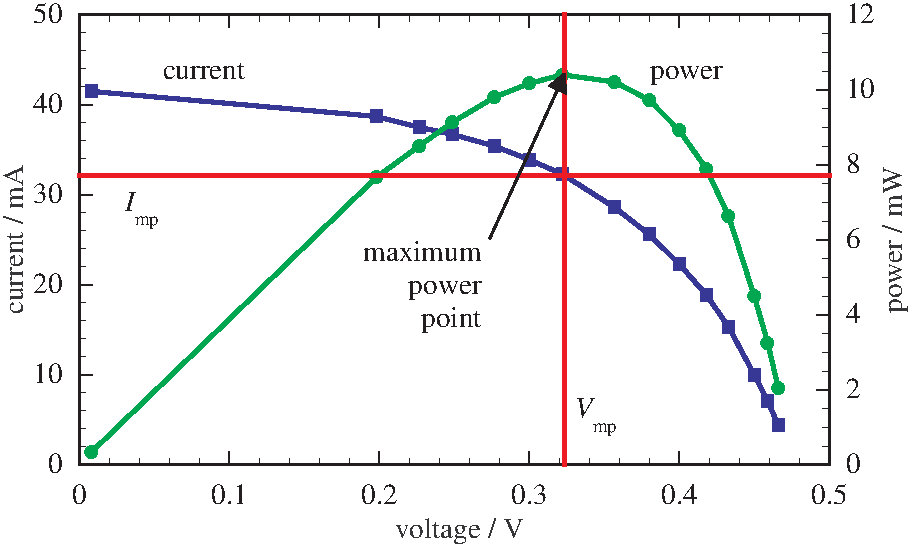
\includegraphics[scale=0.72]{solarcell}
\caption{Current and power as a function of voltage delivered by a single photovoltaic cell under illumination from a 150\,W metal halide floodlamp, showing the maximum power point.}
\label{solar cell fig}
\end{figure}

Figures and tables must have informative captions and be numbered as in Figure~\ref{solar cell fig}. Axes of graphs should have scales, titles and units, otherwise the plot is meaningless. All text must be legible, roughly the same size as the main text. Be warned that plots from Excel need extensive editing to bring them up to an acceptable standard. Oscilloscope screenshots can make good illustrations and are simple to capture on modern equipment.

Tables must have appropriate headings with units. Avoid lengthy tables: consider whether a graph would be clearer or the data would be better on a CD.

\subsection{References}

No project is done in isolation. A research project builds on the results of previous workers; a design-and-build project depends on the properties of the components available. You therefore draw on published documents during your project and must provide \emph{references} to these sources in your report. References are cited (a)~to give due credit to the originator and (b)~to guide a reader who wants more detailed information. You should give a reference wherever it is required for either of these purposes. Properly referenced material from many sources is a sign of a good project report. 
%This section explains how to present such references and how you will be penalised if you fail to do this. The mark for the report include an element for references to reflect their importance.

References must be cited with sequential numbers in square brackets where they are used in the text, not just listed at the end of the report. Typical usage is `Fitzmaurice and Hand \cite{gmf87} showed that\dots' or `The median is an appropriate estimator for this signal \cite{gmf87}'.

Avoid direct quotations from references in general; make it absolutely clear that the text is a quotation if this is unavoidable. An illustration, such as a diagram from a data sheet, is another type of quotation and must be referenced, typically in the figure caption. This is perfectly acceptable: do not waste time redrawing diagrams.

\subsubsection{Plagiarism}

If you copy from another person's work (project report, book, journal, web page or any other document) without acknowledging the source, you are guilty of \emph{plagiarism}. This is a disciplinary offence and the University has procedures for handling it. The failure to acknowledge a source is considered as plagiarism even if there was no deliberate intention to cheat. 

Avoid any risk of plagiarism by providing a reference for all sources that you use. Read the advice offered by the University Library and consult your supervisor if you are in any doubt. The University's \emph{Plagiarism Statement} is reproduced in Appendix \ref{plagiarism sect}.

\subsubsection{List of references}

All reports must have a section entitled `References' after the main text but before any appendices. This comprises a list of references, numbered to match the citations in the text. Each reference requires the following information and the cited references provide examples.
\begin{itemize}
\item
\textbf{Journal paper}: 
author(s), title of paper, name of journal, volume number, first page, last page and year \cite{gmf87}. 
Many journals now use article numbers instead of page numbers.
\item
\textbf{Book}: 
author(s), title, edition, publisher and year of publication \cite{jve05}.
Include the number of the chapter or page(s) if you refer to only a small part of the book.
\item
\textbf{Data sheet}: 
company, title, edition and date \cite{s08qg}. 
Application notes, technical reports and similar documents should be cited in the same way.
\item
\textbf{Web page}: 
author(s) or organisation, title, full URL and date of viewing \cite{mac09}. See below.
\end{itemize}
%The general rule is that 
The reader must be able to find the document without searching for further information.

\subsubsection{References from the Web}

The World Wide Web is a wonderful resource because it is so easy to search. It is therefore tempting to use web pages as references. \emph{Proceed with caution} because the accuracy of many web sites cannot be verified. This is particularly true for anonymous sites such as Wikipedia. Use them only as a starting point: good pages provide references to more authoritative sources.

Reports whose references are all or mainly from the web, especially from anonymous sites, will be penalised.


\section{Discussion}

The discussion is your opportunity to impress an expert with your depth of understanding. Don't worry so much about the non-expert reader -- she or he can skip to the Conclusions.

For a research project this section should provide a logical argument leading from the experimental observations to the final conclusions. Evaluate your results thoroughly and gain every possible piece of understanding from them. Compare the results in detail to other work in the field. This should be a \emph{critical} comparison so don't just say that your results are different from previous work; explain \emph{why}. Never say `The results were as expected' unless you have already described exactly what was expected!

The main purpose of the Discussion in a design-and-build project is to assess the performance of your product against the specification, showing its strengths and weaknesses.


\section{Conclusions}

Every report must have conclusions, built on the discussion. This section includes a summary of the main achievements of the work but is more than that. The noun `conclusion' can be defined as `a judgement or decision reached by reasoning' \cite{oupconc} so you should highlight what has been learnt as a result of your project. What is the big picture that the reader should take away? 

The Conclusions should include an assessment of the outcome against the original aims of the project. If you were unable to fulfil some aims, explain why. It is also useful to review the project plan (which should be included with the report). Did some tasks prove to be unexpectedly difficult, for instance?

\subsection{Suggestions for further work}

Almost every project leaves you with ideas for the future. Research typically answers some questions while opening new ones; by the end of a design-and-build project you may have thought of a superior approach. Examiners are impressed by intelligent suggestions for further work because they show that you really understand the project. It is often a sign of strength to identify the weak points and suggest solutions for them.


\clearpage % start appendices on a new page
\begin{thebibliography}{9}
%\addcontentsline{toc}{section}{References}
\bibitem{jve05}
Joan van Emden,
\textit{Writing for Engineers},
3rd Edition,
Palgrave Macmillan 
(2005).

\bibitem{mkm06}
Marun K. Mitra,
\textit{Effective Technical Communication: A Guide for Scientists and Engineers},
Oxford
(2006).

\bibitem{dfb09}
David F. Beer and David McMurrey,
\textit{A Guide to Writing as an Engineer},
3rd Edition,
Wiley
(2009).

\bibitem{tmy05}
Trevor M. Young,
\textit{Technical Writing A--Z: A Commonsense Guide to Engineering Reports and Theses},
American Society of Mechanical Engineers
(2005).

\bibitem{ronneberger2015unet}
O. Ronneberger, P. Fischer, and T. Brox,
\textit{U-Net: Convolutional networks for biomedical image segmentation},
in \textit{Proc. Medical Image Computing and Computer-Assisted Intervention (MICCAI)},
pp. 234--241,
2015.

\bibitem{isensee2021nnunet}
F. Isensee, P. F. Jaeger, S. A. A. Kohl, J. Petersen, and K. H. Maier-Hein,
\textit{nnU-Net: A self-configuring method for deep learning-based biomedical image segmentation},
Nature Methods,
\textbf{18},
203--211
(2021).

\bibitem{staal2004drive}
J. Staal, M. D. Abramoff, M. Niemeijer, M. A. Viergever, and B. van Ginneken,
\textit{Ridge-based vessel segmentation in color images of the retina},
IEEE Transactions on Medical Imaging,
\textbf{23}(4),
501--509
(2004).

\bibitem{hoover2000locating}
A. Hoover, V. Kouznetsova, and M. Goldbaum,
\textit{Locating blood vessels in retinal images by piecewise threshold probing of a matched filter response},
IEEE Transactions on Medical Imaging,
\textbf{19}(3),
203--210
(2000).

\bibitem{fraz2012ensemble}
M. M. Fraz, A. R. Rudnicka, C. G. Owen, and S. A. Barman,
\textit{An ensemble classification-based approach applied to retinal blood vessel segmentation},
IEEE Transactions on Biomedical Engineering,
\textbf{59}(9),
2538--2548
(2012).

\bibitem{budai2013robust}
A. Budai, R. Bock, A. Maier, J. Hornegger, and G. Michelson,
\textit{Robust vessel segmentation in fundus images},
International Journal of Biomedical Imaging,
\textbf{2013},
154860
(2013).

\bibitem{luo2025panet}
X. Luo, L. Peng, Z. Ke, J. Lin, and Z. Yu,
\textit{PA-Net: A hybrid architecture for retinal vessel segmentation},
Pattern Recognition,
\textbf{161},
111254
(2025).

\bibitem{lee2015dsn}
C.-Y. Lee, S. Xie, P. Gallagher, Z. Zhang, and Z. Tu,
\textit{Deeply-supervised nets},
in \textit{Proc. Artificial Intelligence and Statistics (AISTATS)},
pp. 562--570,
2015.

\bibitem{zhu2021deformabledetr}
X. Zhu, W. Su, L. Lu, B. Li, X. Wang, and J. Dai,
\textit{Deformable DETR: Deformable transformers for end-to-end object detection},
in \textit{Proc. International Conference on Learning Representations (ICLR)},
2021.

\bibitem{zhu2019dcnv2}
X. Zhu, H. Hu, S. Lin, and J. Dai,
\textit{Deformable ConvNets v2: More deformable, better results},
in \textit{Proc. IEEE/CVF Conference on Computer Vision and Pattern Recognition (CVPR)},
pp. 9308--9316,
2019.

\bibitem{hou2021coordatt}
Q. Hou, D. Zhou, and J. Feng,
\textit{Coordinate attention for efficient mobile network design},
in \textit{Proc. IEEE/CVF Conference on Computer Vision and Pattern Recognition (CVPR)},
pp. 13713--13722,
2021.

\bibitem{qi2023dsc}
J. Qi, Y. He, Y. Liu, and X. Xu,
\textit{Dynamic snake convolution based on topological geometric constraints for tubular structure segmentation},
in \textit{Proc. IEEE/CVF International Conference on Computer Vision (ICCV)},
pp. 6070--6079,
2023.

\bibitem{gmf87}
G M Fitzmaurice and D J Hand, 
\textit{A comparison of two average conditional error estimators}, 
Pattern Recognition Letters, 
\textbf{6}, 
221--228 
(1987).

\bibitem{s08qg}
Freescale Semiconductor,
\textit{Datasheet for MC9S08QG microcontroller},
revision 4
(2008).

\bibitem{mac09}
Morgan Advanced Ceramics, 
\textit{Advanced Ceramics: Silicon Nitride}, \texttt{www.morgantechnicalceramics.com} 
(viewed 2009 May 13).

\bibitem{oupconc}
Oxford University Press, 
\textit{AskOxford},
\texttt{www.askoxford.com/?view=uk}
(viewed 2009 May 13).

`Conclusion' is defined as (1)~an end or finish, (2)~the summing-up of an argument or text, (3)~a judgement or decision reached by reasoning or (4)~the settling of a treaty or agreement.
\end{thebibliography}

\clearpage % start appendices on a new page
\appendix

\section{Appendices}

Use appendices for supporting material which is relevant but of a detailed nature. In this way the flow of ideas in the body of the report is not interrupted. Appendices are usually lettered rather than numbered to distinguish them. Several uses for appendices have been suggested already but bear in mind that a CD may be more appropriate for large tables of results, long programs and data sheets or other background information. Appendices are not included in the word count because the assessors are not obliged to read them. Do not put vital points here!

Include your project plan and interim reports as appendices on paper.

\section{University's Plagiarism Statement}
\label{plagiarism sect}

The University's degrees and other academic awards are given in recognition of a student's personal achievement. All work submitted by students for assessment is accepted on the understanding that it is the student's own effort. 

Plagiarism is defined as the submission or presentation of work, in any form, which is not one's own, without acknowledgement of the sources. Plagiarism includes inappropriate collaboration with others. Special cases of plagiarism can arise from a student using his or her own previous work (termed auto-plagiarism or self-plagiarism). Autoplagiarism includes using work that has already been submitted for assessment at this University or for any other academic award.

The incorporation of material without formal and proper acknowledgement (even with no deliberate intent to cheat) can constitute plagiarism. Work may be considered to be plagiarised if it consists of: 
\begin{itemize}
\item
a direct quotation; 
\item
a close paraphrase; 
\item
an unacknowledged summary of a source; 
\item
direct copying or transcription.
\end{itemize}
With regard to essays, reports and dissertations, the rule is: if information or ideas are obtained from any source, that source must be acknowledged according to the appropriate convention in that discipline; and any direct quotation must be placed in quotation marks and the source cited immediately. Any failure to acknowledge adequately or to cite properly other sources in submitted work is plagiarism. Under examination conditions, material learnt by rote or close paraphrase will be expected to follow the usual rules of reference citation otherwise it will be considered as plagiarism. Departments should provide guidance on other appropriate use of references in examination conditions. 

Plagiarism is considered to be an act of fraudulence and an offence against University discipline. Alleged plagiarism, at whatever stage of a student's studies, whether before or after graduation, will be investigated and dealt with appropriately by the University.

The University reserves the right to use plagiarism detection systems, which may be externally based, in the interests of improving academic standards when assessing student work.

\end{document}
